\usetikzlibrary{patterns}

\usetikzlibrary{arrows}
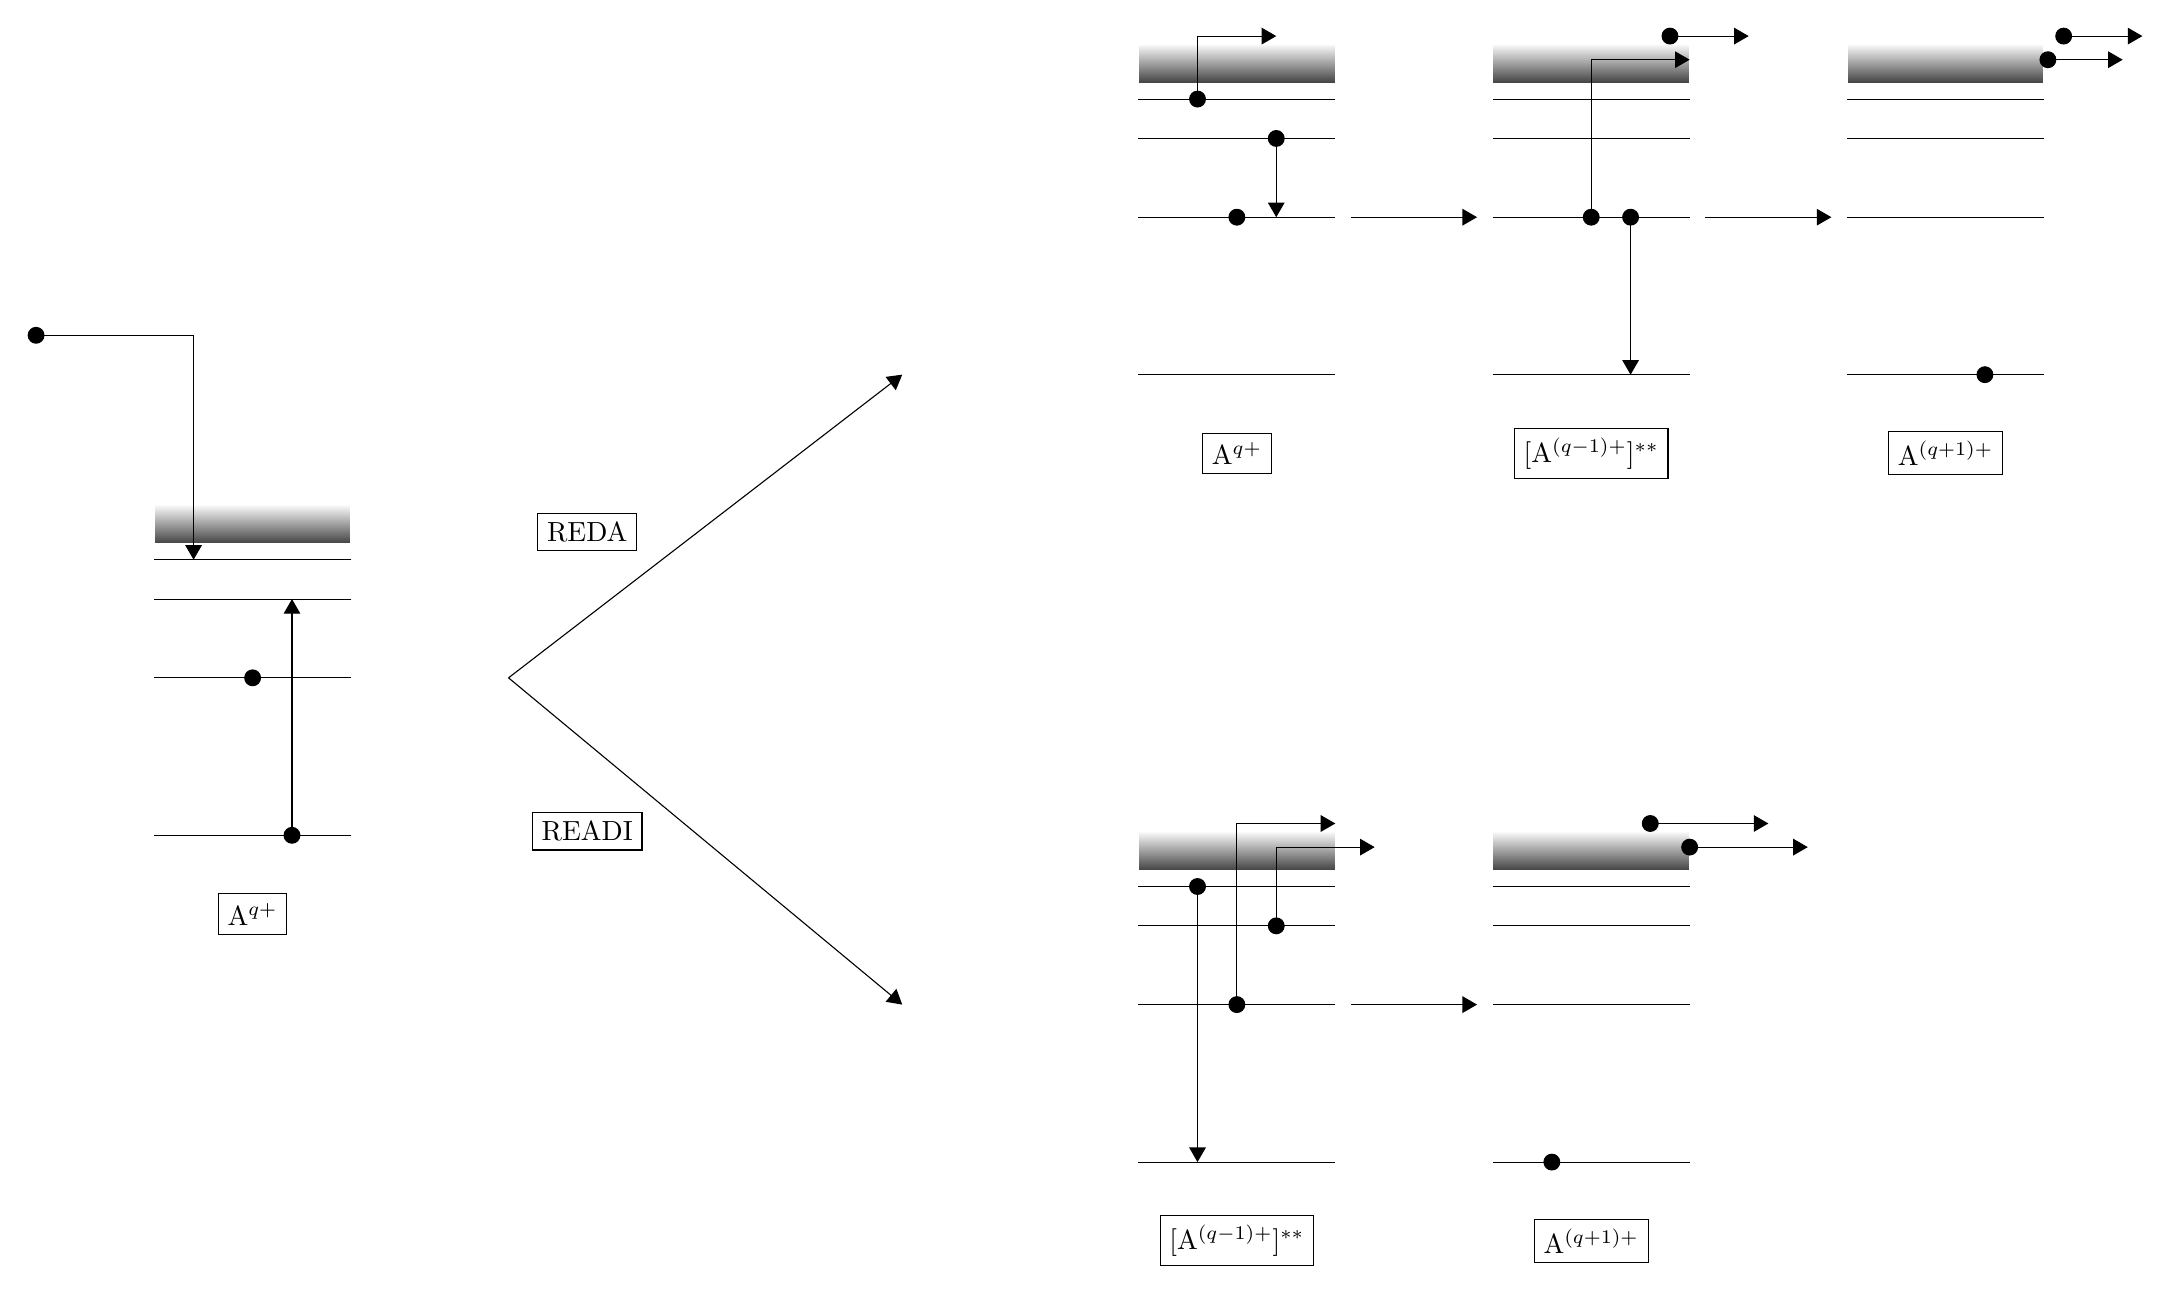
\begin{tikzpicture}
% Anker
%\draw  (-12.5,4.15) ellipse (1 and 1); % Anker Start
%\draw  (0,10) ellipse (1 and 1); % Anker REDA
%\draw  (0,0) ellipse (1 and 1); % Anker READI

%%%%%%%%%%%%%%%%%%%%%%%%%-- Beschriftung --%%%%%%%%%%%%%%%%%%%%%%%%%%%%%
%%%%%%%%%%%%%%%%%%%%%%%%%%%%%%%%%%%%%%%%%%%%%%%%%%%%%%%%%%%%%%%
% Beschriftung
%%% Für Start
\node[draw] at (-11.25,3.15) {A$^{q+}$}; % 1
% Beschriftung
%%% Für REDA
\node[draw] at (1.25,9) {A$^{q+}$}; % 1
\node[draw] at (5.75,9) {[A$^{(q-1)+}$]$^{**}$}; % 2
\node[draw] at (10.25,9) {A$^{(q+1)+}$}; % 3
\node[draw] at (-7,8) {REDA}; % REDA
% Beschriftung
%%% Für READI
\node[draw] at (1.25,-1) {[A$^{(q-1)+}$]$^{**}$}; % 1
\node[draw] at (5.75,-1) {A$^{(q+1)+}$}; % 2
\node[draw] at (-7,4.2) {READI}; % READI
%%%%%%%%%%%%%%%%%%%%%%%%%%%%%%%%%%%%%%%%%%%%%%%%%%%%%%%%%%%%%%%
%%%%%%%%%%%%%%%%%%%%%%%%%%%%%%%%%%%%%%%%%%%%%%%%%%%%%%%%%%%%%%%


%%%%%%%%%%%%%%%%%%%%%%%%%-- Standard Darstellung --%%%%%%%%%%%%%%%%%%%%%%%%
%%%%%%%%%%%%%%%%%%%%%%%%%%%%%%%%%%%%%%%%%%%%%%%%%%%%%%%%%%%%%%%
%%%%%%%%%%%%%%%%%%%%%%%%%%%%%%%%%%%%%%%%%%%%%%%%%%%%%%%%%%%%%%%
%%% Start
% Nr 1 Standard Darstellung ohne Elektronen
%\draw[red] (-12.5,-2.5) --(-12.5,15); % Anker für Mitte y //
%\draw[red] (-12.5,6.25) --(12.5,6.25); % Anker für Mitte x //
\draw (-10,4.15) -- (-12.5,4.15);
\draw (-10,6.15) -- (-12.5,6.15);
\draw (-10,7.15) -- (-12.5,7.15);
\draw (-10,7.65) -- (-12.5,7.65);
\shadedraw [draw=white,top color=lightgray!5,bottom color=darkgray] (-10,7.85) rectangle (-12.5,8.35);
%%%%%%%%%%%%%%%%%%%%%%%%%%%%%%%%%%%%%%%%%%%%%%%%%%%%%%%%%%%%%%%
%%%%%%%%%%%%%%%%%%%%%%%%%%%%%%%%%%%%%%%%%%%%%%%%%%%%%%%%%%%%%%%
%%% Für REDA
% Nr 1 Standard Darstellung ohne Elektronen
\draw (0,10) -- (2.5,10);
\draw (0,12) -- (2.5,12);
\draw (0,13) -- (2.5,13);
\draw (0,13.5) -- (2.5,13.5);
\shadedraw [draw=white,top color=lightgray!5,bottom color=darkgray] (0,13.7) rectangle (2.5,14.2);
% Nr 2 Standard Darstellung ohne Elektronen
\draw (4.5,10) -- (7,10);
\draw (4.5,12) -- (7,12);
\draw (4.5,13) -- (7,13);
\draw (4.5,13.5) -- (7,13.5);
\shadedraw [draw=white,top color=lightgray!5,bottom color=darkgray] (4.5,13.7) rectangle (7.0,14.2);
% Nr 3 Standard Darstellung ohne Elektronen
\draw (9,10) -- (11.5,10);
\draw (9,12) -- (11.5,12);
\draw (9,13) -- (11.5,13);
\draw (9,13.5) -- (11.5,13.5);
\shadedraw [draw=white,top color=lightgray!5,bottom color=darkgray] (9.0,13.7) rectangle (11.5,14.2);
%%%%%%%%%%%%%%%%%%%%%%%%%%%%%%%%%%%%%%%%%%%%%%%%%%%%%%%%%%%%%%%
%%%%%%%%%%%%%%%%%%%%%%%%%%%%%%%%%%%%%%%%%%%%%%%%%%%%%%%%%%%%%%%
%%% Für READI
% Nr 1 Standard Darstellung ohne Elektronen
\draw (0,0) -- (2.5,0);
\draw (0,2) -- (2.5,2);
\draw (0,3) -- (2.5,3);
\draw (0,3.5) -- (2.5,3.5);
\shadedraw [draw=white,top color=lightgray!5,bottom color=darkgray] (0,3.7) rectangle (2.5,4.2);
% Nr 2 Standard Darstellung ohne Elektronen
\draw (4.5,0) -- (7,0);
\draw (4.5,2) -- (7,2);
\draw (4.5,3) -- (7,3);
\draw (4.5,3.5) -- (7,3.5);
\shadedraw [draw=white,top color=lightgray!5,bottom color=darkgray] (4.5,3.7) rectangle (7.0,4.2);
%%%%%%%%%%%%%%%%%%%%%%%%%%%%%%%%%%%%%%%%%%%%%%%%%%%%%%%%%%%%%%%
%%%%%%%%%%%%%%%%%%%%%%%%%%%%%%%%%%%%%%%%%%%%%%%%%%%%%%%%%%%%%%%


%%%%%%%%%%%%%%%%%%%%%%%%%%%%%-- Pfeile --%%%%%%%%%%%%%%%%%%%%%%%%%%%%
%%%%%%%%%%%%%%%%%%%%%%%%%%%%%%%%%%%%%%%%%%%%%%%%%%%%%%%%%%%%%%%
%%%%%%%%%%%%%%%%%%%%%%%%%%%%%%%%%%%%%%%%%%%%%%%%%%%%%%%%%%%%%%%
%%% Für Start
% Pfeile
\draw[-triangle 60] (-8,6.15) -- (-3,10); % nach REDA
\draw[-triangle 60] (-8,6.15) -- (-3,2); % nach READI
%%%%%%%%%%%%%%%%%%%%%%%%%%%%%%%%%%%%%%%%%%%%%%%%%%%%%%%%%%%%%%%
%%%%%%%%%%%%%%%%%%%%%%%%%%%%%%%%%%%%%%%%%%%%%%%%%%%%%%%%%%%%%%%
%%% Für REDA
% Pfeile
\draw[-triangle 60] (2.7,12) -- (4.3,12); % 1 nach 2
\draw[-triangle 60] (7.2,12) -- (8.8,12); % 2 nach 3
%%%%%%%%%%%%%%%%%%%%%%%%%%%%%%%%%%%%%%%%%%%%%%%%%%%%%%%%%%%%%%%
%%%%%%%%%%%%%%%%%%%%%%%%%%%%%%%%%%%%%%%%%%%%%%%%%%%%%%%%%%%%%%%
%%% Für READI
% Pfeile
\draw[-triangle 60] (2.7,2) -- (4.3,2); % 1 nach 2
%%%%%%%%%%%%%%%%%%%%%%%%%%%%%%%%%%%%%%%%%%%%%%%%%%%%%%%%%%%%%%%


%%%%%%%%%%%%%%%%%%%%%%%%%%%%%-- Elektronen --%%%%%%%%%%%%%%%%%%%%%%%%%%
%%%%%%%%%%%%%%%%%%%%%%%%%%%%%%%%%%%%%%%%%%%%%%%%%%%%%%%%%%%%%%%
%%%%%%%%%%%%%%%%%%%%%%%%%%%%%%%%%%%%%%%%%%%%%%%%%%%%%%%%%%%%%%%
%%% Für Start
% Elektronen (von unten nach oben)
% Nr 1 Standard
\filldraw  (-10.75,4.15) ellipse (0.1 and 0.1);
\filldraw  (-11.25,6.15) ellipse (0.1 and 0.1);
\filldraw  (-14,10.5) ellipse (0.1 and 0.1); %Kontinuum Elektron
%%%%%%%%%%%%%%%%%%%%%%%%%%%%%%%%%%%%%%%%%%%%%%%%%%%%%%%%%%%%%%%
%%%%%%%%%%%%%%%%%%%%%%%%%%%%%%%%%%%%%%%%%%%%%%%%%%%%%%%%%%%%%%%
%%%%%%%%%%%%%%%%%%%%%%%%%%%%%%%%%%%%%%%%%%%%%%%%%%%%%%%%%%%%%%%
%%% Für REDA
% Elektronen (von unten nach oben)
% Nr 1 Standard
\filldraw  (1.25,12.0) ellipse (0.1 and 0.1);
\filldraw  (1.75,13.0) ellipse (0.1 and 0.1);
\filldraw  (0.75,13.5) ellipse (0.1 and 0.1); % erstes abgelöstes Elektronen
% Elektronen (von unten nach oben)
% Nr 2 Standard
\filldraw  (6.25,12.0) ellipse (0.1 and 0.1);
\filldraw  (5.75,12.0) ellipse (0.1 and 0.1);
\filldraw  (6.75,14.3) ellipse (0.1 and 0.1); % erstes abgelöstes Elektronen, frei
% Elektronen (von unten nach oben)
% Nr 3 Standard
\filldraw  (10.75,10.0) ellipse (0.1 and 0.1);
\filldraw  (11.55,14.0) ellipse (0.1 and 0.1); % zweites abgelöstes Elektronen, unten
\filldraw  (11.75,14.3) ellipse (0.1 and 0.1); % erstes abgelöstes Elektronen, oben
%%%%%%%%%%%%%%%%%%%%%%%%%%%%%%%%%%%%%%%%%%%%%%%%%%%%%%%%%%%%%%%
%%%%%%%%%%%%%%%%%%%%%%%%%%%%%%%%%%%%%%%%%%%%%%%%%%%%%%%%%%%%%%%
%%% Für READI
% Elektronen (von unten nach oben)
% Nr 1 Standard
\filldraw  (1.25,2.0) ellipse (0.1 and 0.1); % ablösendes Elektron
\filldraw  (1.75,3) ellipse (0.1 and 0.1); % ablösendes Elektron
\filldraw  (0.75,3.5) ellipse (0.1 and 0.1); % fallendes Elektron
% Elektronen (von unten nach oben)
% Nr 2 Standard
\filldraw  (5.25,0) ellipse (0.1 and 0.1); % gefallendes Elektron
\filldraw  (7.0,4.0) ellipse (0.1 and 0.1); % abgelöstes Elektronen, frei unten
\filldraw  (6.5,4.3) ellipse (0.1 and 0.1); % abgelöstes Elektronen, frei oben
%%%%%%%%%%%%%%%%%%%%%%%%%%%%%%%%%%%%%%%%%%%%%%%%%%%%%%%%%%%%%%%
%%%%%%%%%%%%%%%%%%%%%%%%%%%%%%%%%%%%%%%%%%%%%%%%%%%%%%%%%%%%%%%
%%%%%%%%%%%%%%%%%%%%%%%%%%%%%%%%%%%%%%%%%%%%%%%%%%%%%%%%%%%%%%%


%%%%%%%%%%%%%%%%%%%%%%%%%-- Elektronen Weg --%%%%%%%%%%%%%%%%%%%%%%%%%%%
%%%%%%%%%%%%%%%%%%%%%%%%%%%%%%%%%%%%%%%%%%%%%%%%%%%%%%%%%%%%%%%
%%% Für Start
% Elektronenweg
% Nr 1 Standard
\draw [-triangle 60](-14,10.5) -- (-12,10.5) -- (-12,7.65); %Kontinuum Elektron
\draw [-triangle 60](-10.75,4.15) -- (-10.75,7.15); %angeregtes Elektron
%%%%%%%%%%%%%%%%%%%%%%%%%%%%%%%%%%%%%%%%%%%%%%%%%%%%%%%%%%%%%%%
%%%%%%%%%%%%%%%%%%%%%%%%%%%%%%%%%%%%%%%%%%%%%%%%%%%%%%%%%%%%%%%
%%% Für REDA
% Elektronenweg
% Nr 1 Standard
\draw [-triangle 60](1.75,13) -- (1.75,12); % gefallendes Elektron
\draw [-triangle 60](0.75,13.5) -- (0.75,14.3) -- (1.75,14.3); % abgelöstes Elektron
% Nr 2 Standard
\draw [-triangle 60](6.25,12) -- (6.25,10); % gefallendes Elektron
\draw [-triangle 60](5.75,12) -- (5.75,14.0) -- (7.0,14); % ablösendes Elektron
\draw [-triangle 60](6.75,14.3) -- (7.75,14.3); % abgelöstes Elektron
% Nr 3 Standard
\draw [-triangle 60](11.55,14.0) -- (12.5,14.0); % ablösendes Elektron
\draw [-triangle 60] (11.75,14.3) -- (12.75,14.3); % abgelöstes Elektron
%%%%%%%%%%%%%%%%%%%%%%%%%%%%%%%%%%%%%%%%%%%%%%%%%%%%%%%%%%%%%%%
%%%%%%%%%%%%%%%%%%%%%%%%%%%%%%%%%%%%%%%%%%%%%%%%%%%%%%%%%%%%%%%
%%% Für READI
% Elektronenweg
% Nr 1 Standard
\draw [-triangle 60](1.75,3) -- (1.75,4.0) -- (3,4.0); % ablösendes Elektron unten
\draw [-triangle 60](1.25,2) -- (1.25,4.3) -- (2.5,4.3); % ablösendes Elektron oben
\draw [-triangle 60](0.75,3.5) -- (0.75,0); % fallendes Elektron 
% Nr 2 Standard
\draw [-triangle 60](7,4) -- (8.5,4.0); % ablösendes Elektron unten
\draw [-triangle 60](6.5,4.3) --  (8,4.3); % ablösendes Elektron oben 
\end{tikzpicture}